% ============================================================
\chapter{Accuracy, Asymmetric Errors, and Qualitative Results}
\label{ch:results}
% ============================================================

\section{Reference PIDNet-S Result}

Table~\ref{tab:frozen_pidnet_result} reports the retained checkpoint on all 544
official test images. No image subset is used for the aggregate. This
artifact-level measurement is kept separate from the three-seed PIDNet mean,
which comes from a different training protocol.

\begin{table}[H]
\centering
\caption{Verified reference PIDNet-S result for blue+green traversability. Lower
FSR and FBR are preferable; the other quality metrics are higher-is-better.}
\label{tab:frozen_pidnet_result}
\begin{tabular}{@{}lr@{}}
\toprule
\textbf{Metric} & \textbf{Value} \\
\midrule
mIoU & \textbf{0.893941} \\
IoU untraversable & 0.908936 \\
IoU traversable & 0.878946 \\
Traversable precision & 0.941592 \\
Traversable recall & 0.929631 \\
Traversable F1 & 0.935573 \\
False-Safe Rate & \textbf{0.043176} (4.32\%) \\
False-Block Rate & \textbf{0.070369} (7.04\%) \\
Weighted cross-entropy test loss & 0.149528 \\
\bottomrule
\end{tabular}
\end{table}

Untraversable IoU is 3.00 percentage points higher than traversable IoU.
Traversable precision exceeds recall by 1.20 points, and FBR is 2.72 points
higher than FSR. At threshold 0.50, the model is therefore more likely to
remove an annotated traversable pixel than to open an annotated blocked pixel.
That conservative balance is visible numerically, but it does not prevent
large false-safe regions in individual images.

\begin{table}[H]
\centering
\caption{Aggregated pixel confusion matrix for the reference PIDNet-S checkpoint.
Rows are ground truth and columns are prediction.}
\label{tab:frozen_confusion}
\begin{tabular}{@{}llrr@{}}
\toprule
 & & \multicolumn{2}{c}{\textbf{Predicted}} \\
\cmidrule(lr){3-4}
 & & Untraversable & Traversable \\
\midrule
\multirow{2}{*}{\textbf{Ground truth}}
 & Untraversable & 73,151,244 (TN) & \textcolor{safety}{3,300,886 (FP)} \\
 & Traversable & \textcolor{block}{4,027,996 (FN)} & 53,213,314 (TP) \\
\bottomrule
\end{tabular}
\end{table}

Table~\ref{tab:frozen_confusion} exposes the four raw counts from which the
reference checkpoint's aggregate rates are calculated.

The matrix contains exactly
$544\times640\times384=133{,}693{,}440$ pixel decisions. Substitution into
Equations~\ref{eq:final_fsr} and \ref{eq:final_fbr} gives
\begin{align}
 \FSR&=\frac{3{,}300{,}886}{73{,}151{,}244+3{,}300{,}886}=0.043176,\\
 \FBR&=\frac{4{,}027{,}996}{53{,}213{,}314+4{,}027{,}996}=0.070369.
\end{align}
A fresh CPU evaluation reproduced all four counts and every derived metric
exactly. This direct calculation also prevents the two denominators from being
accidentally interchanged.

\section{PIDNet--ROD Comparison}

Under the matched three-seed blue+green recipe, ROD reaches
$0.9138\pm0.0003$ mIoU compared with $0.8822\pm0.0002$ for PIDNet-S. The
reported difference is 3.15 percentage points using the unrounded run values.
ROD also reduces mean FSR from 4.98\% to 3.51\% and mean FBR from 7.67\% to
5.62\%. Under blue-only, ROD reaches $0.9211\pm0.0010$ versus
$0.8832\pm0.0016$ for PIDNet-S, a 3.79-point improvement, while reducing both
asymmetric rates.

The small observed ROD standard deviations and the size of the mean gaps show
that its advantage over PIDNet-S is not explained by one favourable seed: ROD records
the higher test mIoU in every one of the six policy--seed runs. Because
ROD simultaneously changes architecture, pretraining, normalisation, internal
resolution, and trainable-parameter allocation, the experiment does not show
which component causes the improvement. It establishes that the complete ROD
pipeline achieves higher CaT accuracy than the matched PIDNet pipeline.

The closest documented ROD recipe improves further
(Table~\ref{tab:rod_paper_results}). For blue+green, mIoU rises by 0.98 points
over the controlled ROD mean. FSR is 0.34 points higher, but FBR falls by 1.65
points, so much of the gain reflects better recovery of traversable pixels
rather than uniformly more conservative prediction. For blue-only, both
reported error rates improve relative to controlled ROD.

\begin{table}[H]
\centering
\caption{Closest documented ROD recipe transferred to CaT. This is a
single-seed approximation because the publication omits the epoch budget and
augmentation policy.}
\label{tab:rod_paper_results}
\small
\begin{tabular}{@{}lrrrrrr@{}}
\toprule
\textbf{Policy} & \textbf{mIoU} & \textbf{IoU untrav.} & \textbf{IoU trav.} & \textbf{F1} & \textbf{FSR} & \textbf{FBR} \\
\midrule
Blue+green & 0.9236 & 0.9338 & 0.9134 & 0.9547 & 3.85\% & 3.97\% \\
Blue-only & 0.9280 & 0.9590 & 0.8970 & 0.9457 & 2.20\% & 5.14\% \\
\bottomrule
\end{tabular}
\end{table}

These experiments establish a repeatable advantage over PIDNet-S. Whether that
advantage is competitive with other compact systems is answered by the
nine-model comparison.

\section{Fixed-Budget Blue+Green Architecture Comparison}

Table~\ref{tab:wider_blue_green} gives the nine-model result for the
blue+green policy after the original common budget of 15 epochs. The FPN with
an EfficientNet-B0 encoder has the highest
observed mean mIoU at 93.15\%; the corresponding U-Net records 93.13\%.
Both have a population standard deviation of 0.07 percentage points across
the three runs, whereas their means differ by only 0.02 points. With only
three runs, the data support a common leading performance band but not a
reliable ordering of the two decoders.

\begin{table}[H]
\centering
\caption{Fixed-15-epoch blue+green results over seeds 1337, 2027, and 4242
(mean $\pm$ population standard deviation). Lower FSR and FBR are preferable.}
\label{tab:wider_blue_green}
\footnotesize
\setlength{\tabcolsep}{4pt}
\begin{tabular}{@{}lrrrr@{}}
\toprule
\textbf{Model} & \textbf{mIoU} & \textbf{F1} & \textbf{FSR} & \textbf{FBR} \\
\midrule
\textbf{FPN/EfficientNet-B0} & $\mathbf{0.9315\pm0.0007}$ & $\mathbf{0.9594\pm0.0005}$ & $0.0293\pm0.0013$ & $\mathbf{0.0420\pm0.0021}$ \\
\textbf{U-Net/EfficientNet-B0} & $\mathbf{0.9313\pm0.0007}$ & $\mathbf{0.9592\pm0.0004}$ & $\mathbf{0.0288\pm0.0007}$ & $0.0429\pm0.0016$ \\
FPN/MobileNetV2 & $0.9255\pm0.0001$ & $0.9556\pm0.0001$ & $0.0309\pm0.0013$ & $0.0472\pm0.0015$ \\
SegFormer-B0 & $0.9254\pm0.0002$ & $0.9555\pm0.0001$ & $0.0296\pm0.0008$ & $0.0491\pm0.0009$ \\
U-Net/MobileNetV2 & $0.9207\pm0.0016$ & $0.9528\pm0.0009$ & $0.0374\pm0.0029$ & $0.0446\pm0.0019$ \\
ROD ViT-S & $0.9138\pm0.0003$ & $0.9482\pm0.0003$ & $0.0351\pm0.0028$ & $0.0562\pm0.0038$ \\
BiSeNetV2 & $0.8868\pm0.0007$ & $0.9307\pm0.0005$ & $0.0425\pm0.0039$ & $0.0803\pm0.0048$ \\
PIDNet-S & $0.8822\pm0.0002$ & $0.9281\pm0.0002$ & $0.0498\pm0.0043$ & $0.0767\pm0.0053$ \\
DDRNet-23-Slim & $0.8746\pm0.0063$ & $0.9228\pm0.0042$ & $0.0499\pm0.0020$ & $0.0862\pm0.0062$ \\
\bottomrule
\end{tabular}
\end{table}

Relative to PIDNet-S, FPN/EfficientNet-B0 improves mean mIoU by 4.93 points,
reduces FSR by 2.05 points, and reduces FBR by 3.47 points. The gain is not
merely a threshold shift from one error direction to the other. U-Net with the
same encoder has nearly identical accuracy and the lowest observed mean FSR.
FPN has slightly lower FBR. With three seeds, those small differences support
a shared performance tier rather than selecting one decoder universally.

The $2\times2$ encoder--decoder subset shows two consistent patterns.
EfficientNet-B0 improves mean mIoU over MobileNetV2 with either FPN or U-Net,
and FPN improves mean mIoU over U-Net with either encoder. The decoder effect
is much smaller with EfficientNet-B0 than with MobileNetV2. SegFormer-B0 has
nearly the same mean mIoU as FPN/MobileNetV2. ROD ranks sixth in this
controlled table: substantially above PIDNet-S, BiSeNetV2, and DDRNet, but
below the four generic encoder--decoder systems and SegFormer-B0.

The single-seed ROD paper recipe reaches 92.36\%, which narrows the gap but
still remains below the 93.15\% and 93.13\% three-seed means of the top
controlled systems. Since its optimiser, loss, augmentation, and seed protocol
differ, that observation is descriptive rather than a strict row-wise
comparison.

\section{Convergence-Aware Blue+Green Follow-Up}

The fixed-budget table controls training exposure, but it does not show what
the same recipes reach after their validation curves flatten. The follow-up
therefore keeps the blue+green data, loss, augmentation, optimiser, initial
learning rate, threshold, and three seeds fixed while extending the training
horizon. The 300 epochs are a ceiling. No run reaches it: early stopping ends
the 27 runs between epochs 74 and 150, and validation selects checkpoints
between epochs 50 and 141.

Table~\ref{tab:convergence_blue_green} reports the resulting test metrics. The
selected epochs are listed in seed order 1337, 2027, and 4242. They are part of
the result because replacing them with one round number would conceal large
between-model and between-seed differences.

\begin{table}[H]
\centering
\caption[Convergence-aware blue+green architecture results.]{Convergence-aware
blue+green results over seeds 1337, 2027, and 4242. Each metric cell places
the mean above its $\pm$ population standard deviation. ``Selected epochs''
gives the validation-selected \texttt{best.pt} epoch for those three seeds.
Lower FSR and FBR are preferable.}
\label{tab:convergence_blue_green}
\footnotesize
\setlength{\tabcolsep}{4pt}
\renewcommand{\arraystretch}{1.08}
\newcommand{\resultcell}[2]{\shortstack{$#1$\\[-1pt]{\scriptsize$\pm #2$}}}
\begin{tabular*}{\textwidth}{@{\extracolsep{\fill}}lccccc@{}}
\toprule
\textbf{Model} & \textbf{Selected epochs} & \textbf{mIoU} & \textbf{F1} & \textbf{FSR} & \textbf{FBR} \\
\midrule
\textbf{FPN/EfficientNet-B0} & 119/90/83 & \resultcell{\mathbf{0.9423}}{\mathbf{0.0005}} & \resultcell{\mathbf{0.9660}}{\mathbf{0.0003}} & \resultcell{\mathbf{0.0255}}{\mathbf{0.0004}} & \resultcell{\mathbf{0.0340}}{\mathbf{0.0011}} \\
U-Net/EfficientNet-B0 & 102/76/56 & \resultcell{0.9409}{0.0004} & \resultcell{0.9652}{0.0002} & \resultcell{0.0260}{0.0002} & \resultcell{0.0349}{0.0003} \\
FPN/MobileNetV2 & 70/99/65 & \resultcell{0.9372}{0.0005} & \resultcell{0.9629}{0.0003} & \resultcell{0.0274}{0.0003} & \resultcell{0.0376}{0.0010} \\
SegFormer-B0 & 50/141/87 & \resultcell{0.9341}{0.0005} & \resultcell{0.9610}{0.0003} & \resultcell{0.0304}{0.0004} & \resultcell{0.0374}{0.0002} \\
U-Net/MobileNetV2 & 74/79/57 & \resultcell{0.9332}{0.0004} & \resultcell{0.9605}{0.0002} & \resultcell{0.0314}{0.0001} & \resultcell{0.0372}{0.0005} \\
ROD ViT-S & 74/82/54 & \resultcell{0.9331}{0.0004} & \resultcell{0.9604}{0.0002} & \resultcell{0.0294}{0.0005} & \resultcell{0.0399}{0.0003} \\
PIDNet-S & 104/75/75 & \resultcell{0.9195}{0.0029} & \resultcell{0.9519}{0.0018} & \resultcell{0.0335}{0.0013} & \resultcell{0.0511}{0.0019} \\
BiSeNetV2 & 125/58/123 & \resultcell{0.9149}{0.0019} & \resultcell{0.9490}{0.0012} & \resultcell{0.0361}{0.0021} & \resultcell{0.0536}{0.0020} \\
DDRNet-23-Slim & 81/68/93 & \resultcell{0.9095}{0.0022} & \resultcell{0.9456}{0.0014} & \resultcell{0.0374}{0.0009} & \resultcell{0.0584}{0.0017} \\
\bottomrule
\end{tabular*}
\end{table}

FPN/EfficientNet-B0 has the highest mean mIoU and also the lowest mean FSR and
FBR. It scores above U-Net/EfficientNet-B0 in each matched seed; the mean lead
is 0.13 percentage points. This is a consistent first place within the 27
executed runs, although three seeds and one split do not establish a universal
decoder ranking. The two MobileNetV2 decoders separate more clearly:
FPN/MobileNetV2 leads U-Net/MobileNetV2 by 0.41 points. ROD and
U-Net/MobileNetV2 differ by only 0.003 percentage points in mean mIoU, far
below either model's observed between-seed standard deviation, but retain
different error balances.

\begin{figure}[H]
\centering
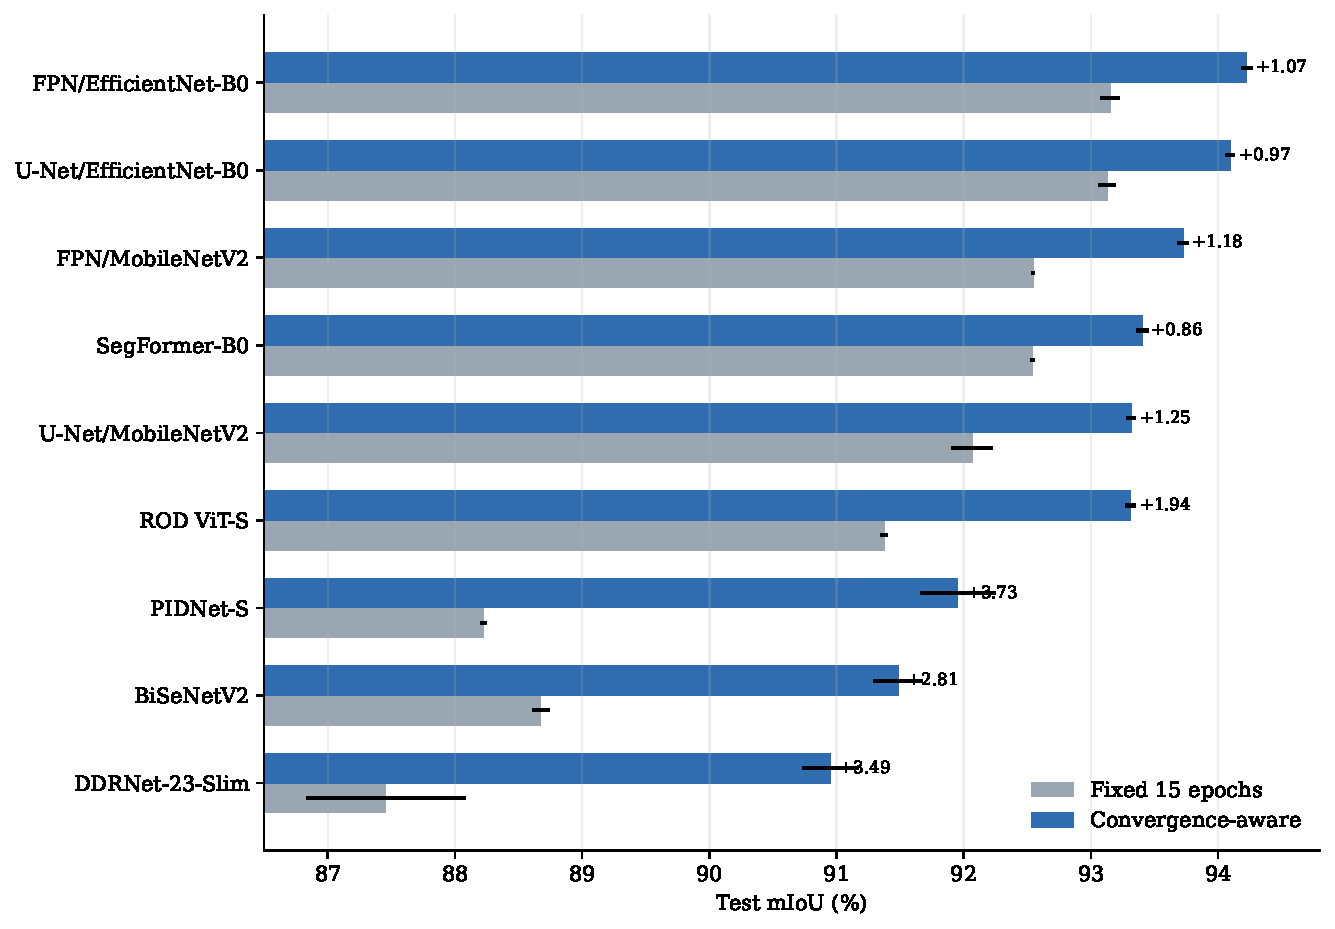
\includegraphics[width=0.98\textwidth]{figures/generated/convergence_miou_comparison.pdf}
\caption[Fixed-budget and convergence-aware test mIoU.]{Mean test mIoU under
the fixed 15-epoch and convergence-aware blue+green protocols. Error bars are
population standard deviations over three seeds; labels give the change in
percentage points. Every architecture improves, but the size of the gain is
strongly model-dependent.}
\label{fig:convergence_miou_comparison}
\end{figure}

Figure~\ref{fig:convergence_miou_comparison} shows that the extended protocol
does not merely add a common offset. PIDNet-S gains 3.73 points,
DDRNet-23-Slim 3.49, and BiSeNetV2 2.81, whereas the two EfficientNet-B0
systems gain about one point. The earlier comparison therefore penalised the
slower-converging real-time models most strongly. Since the follow-up was run
later and used two recorded PyTorch environments across architecture groups,
the exact differences are protocol-level changes rather than pure causal
estimates of additional epochs alone.

\begin{figure}[H]
\centering
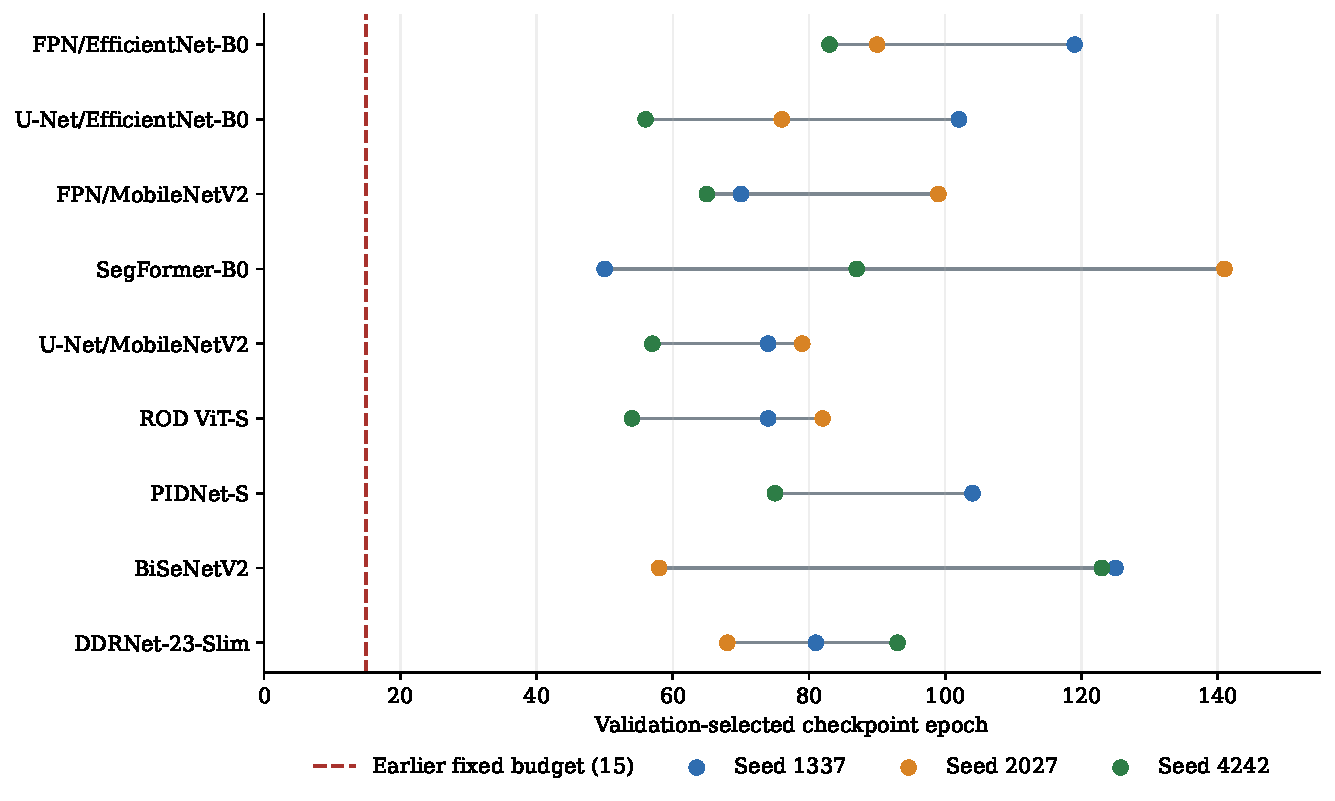
\includegraphics[width=0.98\textwidth]{figures/generated/convergence_selected_epochs.pdf}
\caption[Validation-selected epochs in the convergence suite.]{Checkpoint
epochs selected by validation mIoU. The dashed line marks the earlier
15-epoch budget. Horizontal segments span the three seeds of one architecture;
none of the 27 selected checkpoints lies near epoch 15.}
\label{fig:convergence_selected_epochs}
\end{figure}

Figure~\ref{fig:convergence_selected_epochs} shows both between-model and
between-seed variation in the validation-selected checkpoint epoch.

The selected epochs range from 50 for one SegFormer run to 141 for another.
This spread is the direct reason not to replace the fixed budget with a claim
that one epoch count, such as 60 or 300, is ``optimal'' for every model. The
curves in Figure~\ref{fig:convergence_validation_curves} add the missing
temporal context: pretrained encoder--decoders rise quickly but continue to
make small gains, while PIDNet, BiSeNet, and DDRNet require a longer initial
climb.

\begin{figure}[H]
\centering
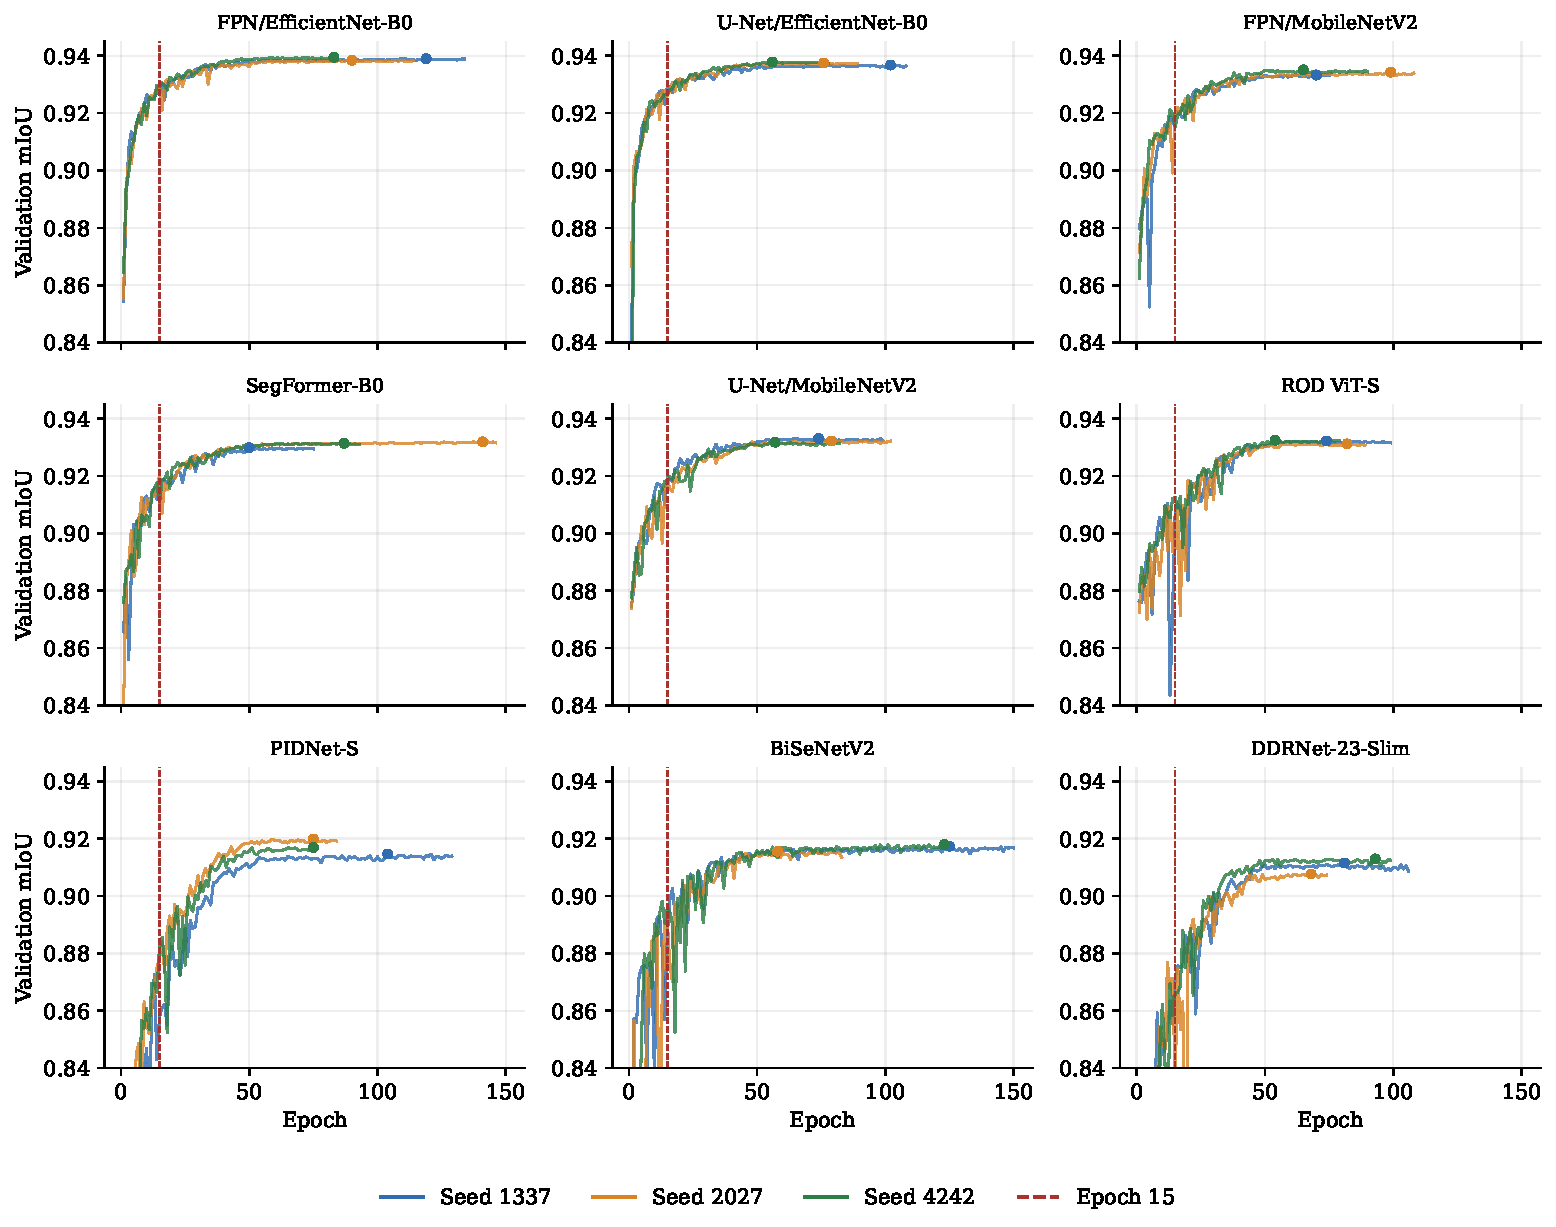
\includegraphics[width=\textwidth]{figures/generated/convergence_validation_curves.pdf}
\caption[Validation histories for the convergence-aware runs.]{Validation
mIoU histories for all 27 convergence-aware runs. Dots mark the saved maximum
for each seed and the dashed line marks epoch 15. The histories support a
longer protocol, but their late fluctuations also show why validation-based
checkpoint selection is preferable to reporting the final epoch.}
\label{fig:convergence_validation_curves}
\end{figure}

\section{Blue-Only Architecture Comparison}

The blue-only table shows the same broad ordering. The task is different, so
its higher mIoU values should not be interpreted as a direct improvement over
blue+green. The EfficientNet-B0 FPN and U-Net again form the top tier: their
means differ by 0.04 points, comparable to their observed 0.05--0.06-point seed
variation.

Table~\ref{tab:wider_blue_only} reports this fixed-budget blue-only matrix in
full; it is not merged with the convergence-aware blue+green evidence.

\begin{table}[H]
\centering
\caption{Controlled blue-only results over seeds 1337, 2027, and 4242
(mean $\pm$ population standard deviation). Lower FSR and FBR are preferable.}
\label{tab:wider_blue_only}
\footnotesize
\setlength{\tabcolsep}{4pt}
\begin{tabular}{@{}lrrrr@{}}
\toprule
\textbf{Model} & \textbf{mIoU} & \textbf{F1} & \textbf{FSR} & \textbf{FBR} \\
\midrule
\textbf{FPN/EfficientNet-B0} & $\mathbf{0.9376\pm0.0006}$ & $\mathbf{0.9531\pm0.0005}$ & $\mathbf{0.0180\pm0.0007}$ & $0.0469\pm0.0016$ \\
\textbf{U-Net/EfficientNet-B0} & $\mathbf{0.9372\pm0.0005}$ & $\mathbf{0.9529\pm0.0004}$ & $0.0192\pm0.0013$ & $\mathbf{0.0445\pm0.0028}$ \\
FPN/MobileNetV2 & $0.9332\pm0.0009$ & $0.9497\pm0.0007$ & $0.0193\pm0.0015$ & $0.0502\pm0.0040$ \\
SegFormer-B0 & $0.9286\pm0.0013$ & $0.9461\pm0.0010$ & $0.0214\pm0.0008$ & $0.0523\pm0.0011$ \\
U-Net/MobileNetV2 & $0.9283\pm0.0001$ & $0.9460\pm0.0000$ & $0.0233\pm0.0017$ & $0.0479\pm0.0040$ \\
ROD ViT-S & $0.9211\pm0.0010$ & $0.9401\pm0.0008$ & $0.0230\pm0.0013$ & $0.0597\pm0.0019$ \\
BiSeNetV2 & $0.8885\pm0.0026$ & $0.9140\pm0.0020$ & $0.0363\pm0.0028$ & $0.0788\pm0.0052$ \\
PIDNet-S & $0.8832\pm0.0016$ & $0.9093\pm0.0014$ & $0.0353\pm0.0016$ & $0.0897\pm0.0039$ \\
DDRNet-23-Slim & $0.8743\pm0.0042$ & $0.9019\pm0.0039$ & $0.0384\pm0.0022$ & $0.0963\pm0.0116$ \\
\bottomrule
\end{tabular}
\end{table}

The best blue-only systems reach lower FSR than under blue+green because the
negative class is larger and the target boundary changes; the numerical rates
remain policy-specific. ROD retains its advantage over PIDNet-S but again ranks
below the five strongest compact alternatives. DDRNet's larger standard
deviation shows that not every architecture is equally stable under the
15-epoch recipe.

For literature context, the reconstructed ROD blue-only traversable IoU is
89.70\%, while the original CaT PSPNet/ResNet-101 sedan IoU is 91.65\%
~\cite{sharma2022cat}. The positive pixel identity is aligned, but one model is
trained as binary segmentation and the other as four-class segmentation, so
the 1.95-point gap is contextual rather than a controlled architecture
comparison.

\section{High-Performing PIDNet Cases}

Figure~\ref{fig:pidnet_successes} presents the four PIDNet cases with the
lowest per-image sum of FSR and FBR. Each triptych shows the RGB image, ground
truth, and prediction. The two open-field examples demonstrate that the
model can reproduce a nearly horizontal transition between a foreground
vehicle-capability region and a distant blocked field even when both are pale
and textured. The wooded-trail example recovers a narrowing corridor and its
asymmetric edges. The curved open-track example follows a broad bend while
leaving a small interior blocked island.

\begin{figure}[H]
\centering

\includegraphics[width=0.48\linewidth]{figures/qualitative/pidnet_success_mixed_pln_1311.png}
\hfill
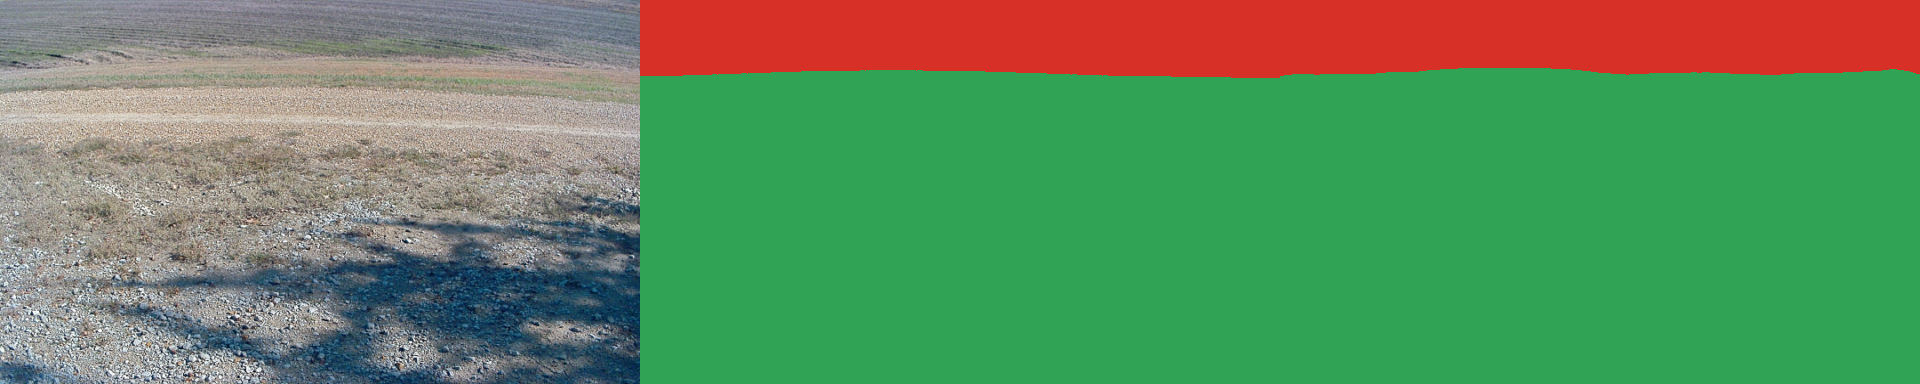
\includegraphics[width=0.48\linewidth]{figures/qualitative/pidnet_success_mixed_pln_1306.png}

\vspace{0.2cm}
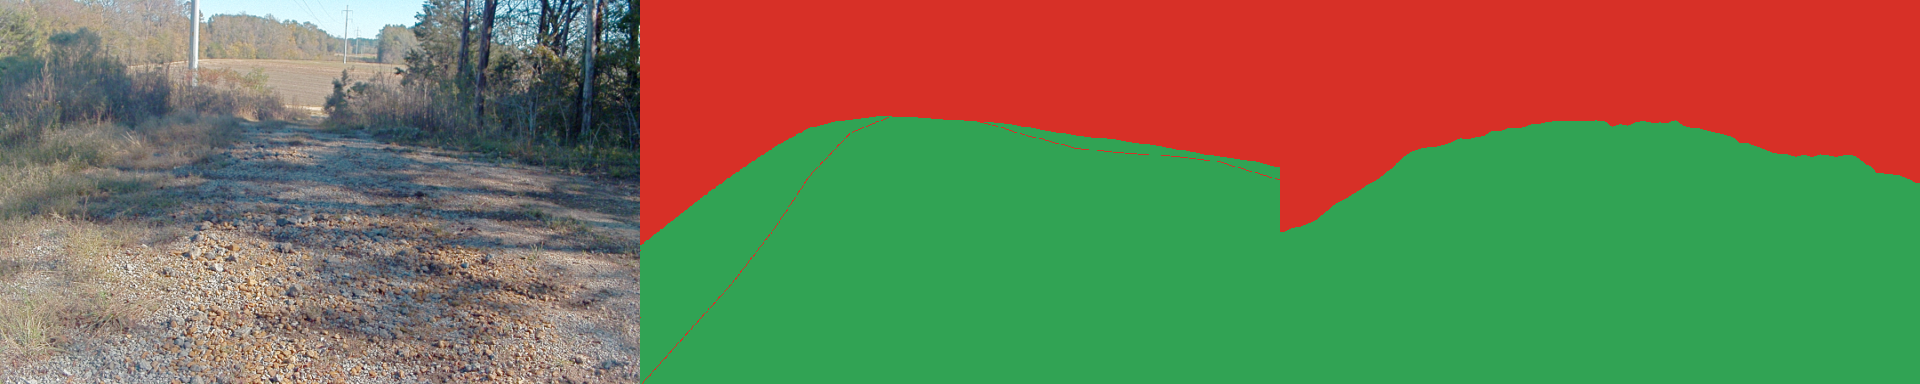
\includegraphics[width=0.48\linewidth]{figures/qualitative/pidnet_success_mixed_pln_1188.png}
\hfill
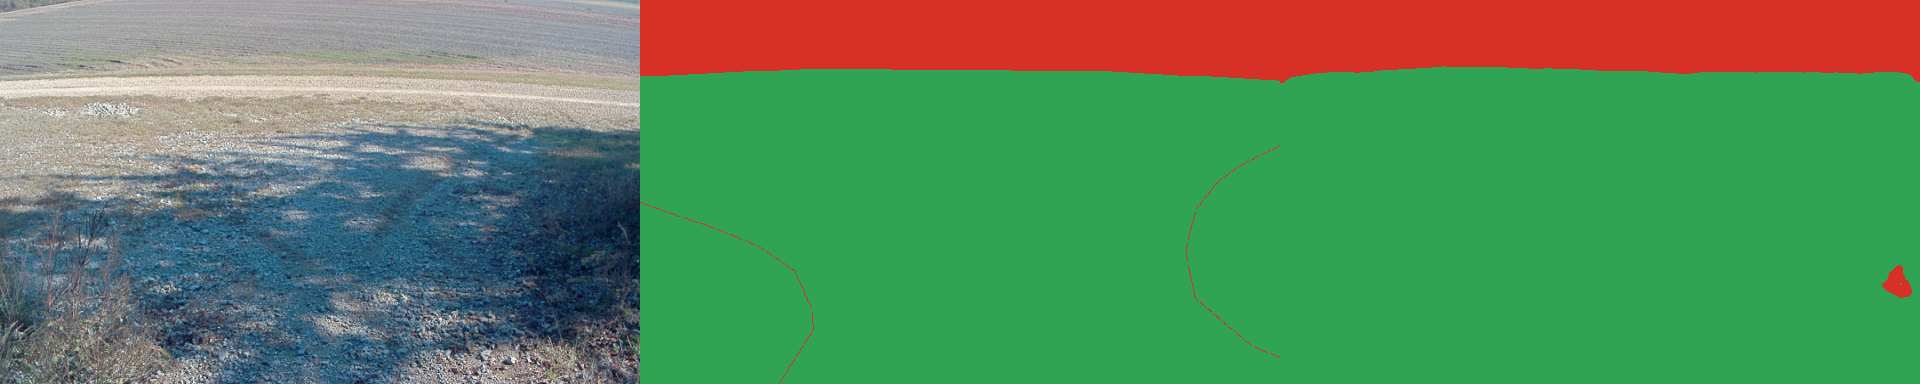
\includegraphics[width=0.48\linewidth]{figures/qualitative/pidnet_success_mixed_pln_1282.png}
\caption[High-performing reference PIDNet-S examples.]{High-performing
reference PIDNet-S examples selected by the lowest per-image sum of FSR and FBR. Each
triptych is RGB, binary ground truth, and prediction. Green denotes
traversable; red denotes untraversable. These are reproducible successes, not
a representative sample of the complete test distribution.}
\label{fig:pidnet_successes}
\end{figure}

The similarity between the ground-truth and prediction panels in these cases
shows that the model is learning a region-level task, not merely detecting a
central road centreline. It predicts the full visible capability envelope and
responds to distant boundary shape. Selection by low error also means these
images cannot be used to infer how often such behaviour occurs.

\section{Performance Across the Test Distribution}

Figure~\ref{fig:pidnet_percentiles} spans the 10th to 90th percentiles of
combined per-image error. The top winding-track image recovers a broad
connected corridor with small contour differences. By the 70th percentile the
prediction narrows the visible region, and the 90th-percentile woodland case
blocks much of a weakly defined corridor.

\begin{figure}[H]
\centering
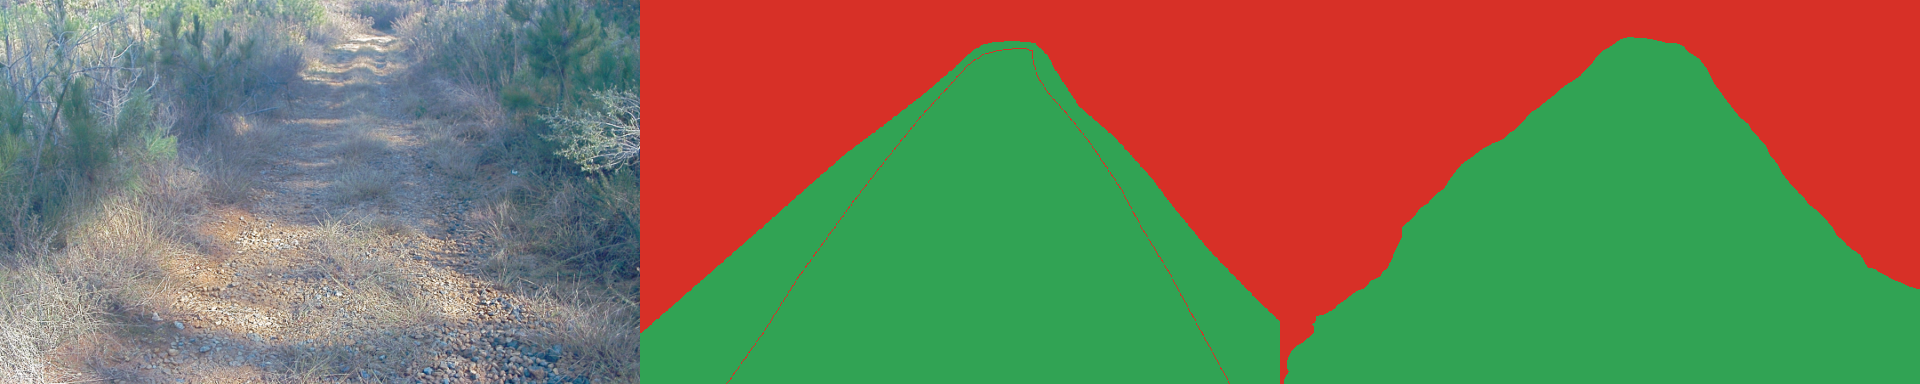
\includegraphics[width=0.96\linewidth]{figures/qualitative/pidnet_percentile_10_mixed_pln_961.png}

\vspace{0.12cm}
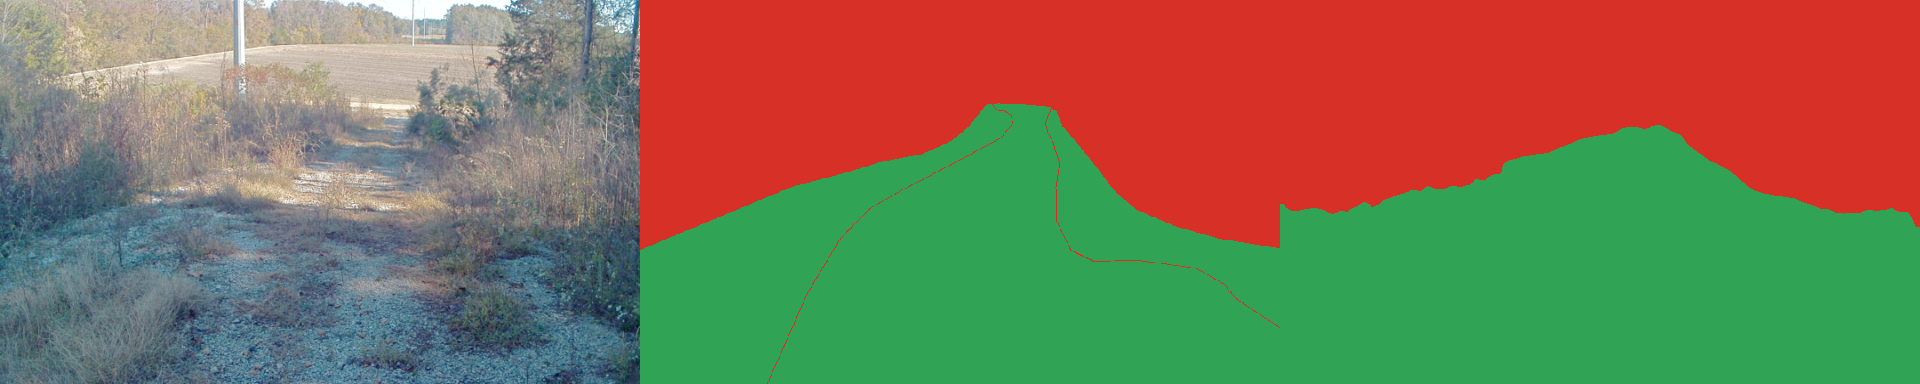
\includegraphics[width=0.96\linewidth]{figures/qualitative/pidnet_percentile_30_mixed_pln_1209.png}

\vspace{0.12cm}
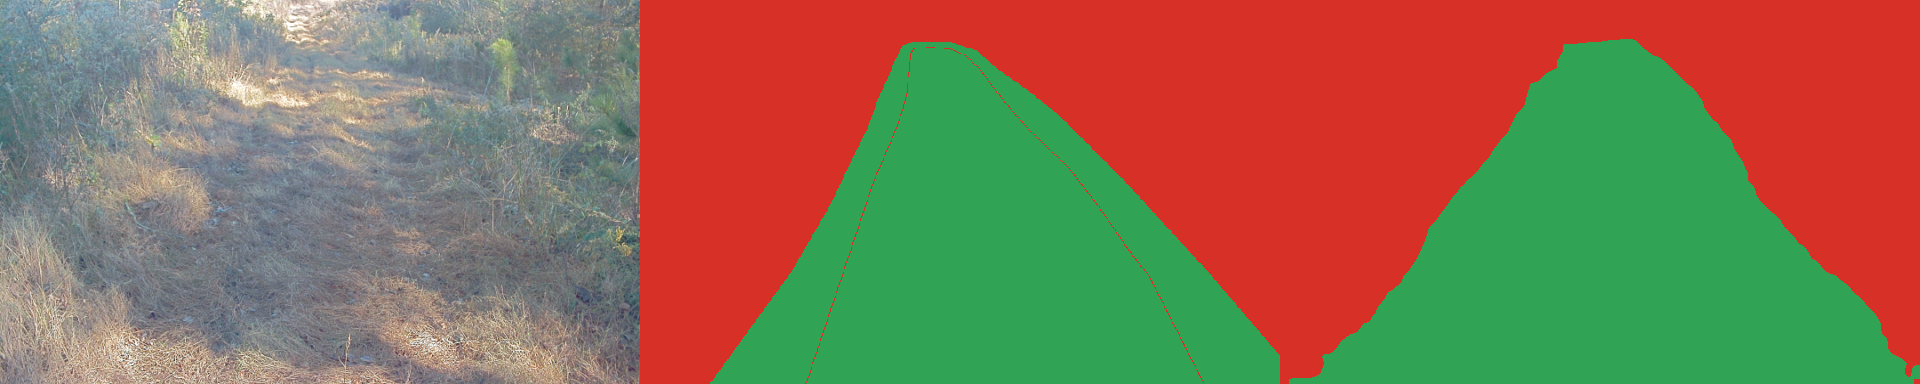
\includegraphics[width=0.96\linewidth]{figures/qualitative/pidnet_percentile_50_mixed_pln_119.png}

\vspace{0.12cm}
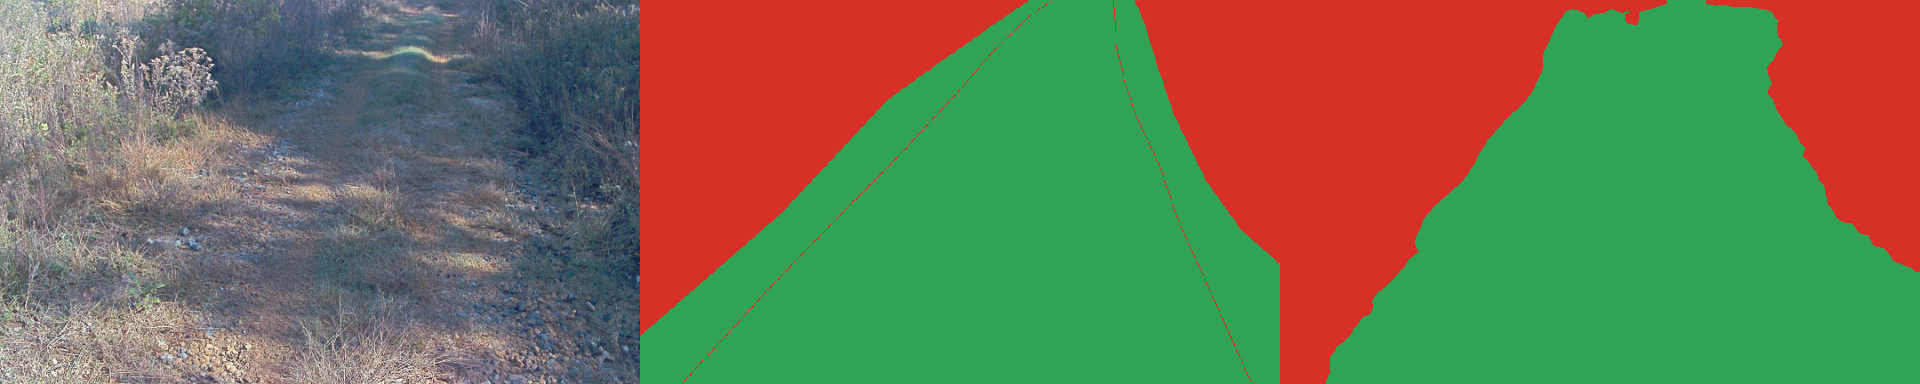
\includegraphics[width=0.96\linewidth]{figures/qualitative/pidnet_percentile_70_mixed_pln_1033.png}

\vspace{0.12cm}
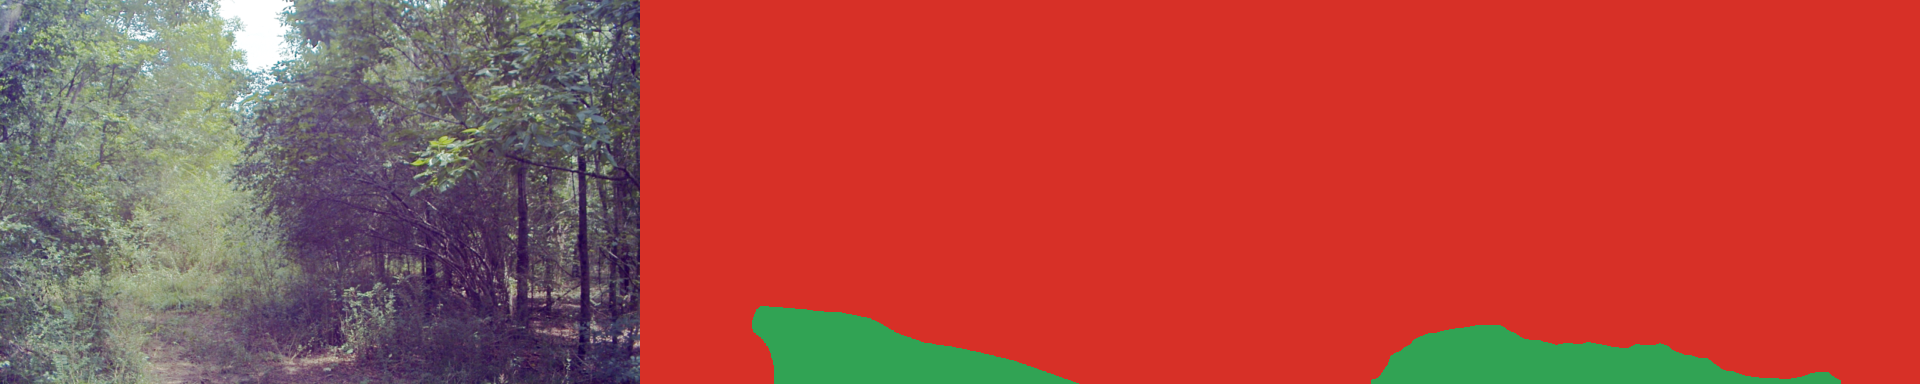
\includegraphics[width=0.96\linewidth]{figures/qualitative/pidnet_percentile_90_mixed_89.png}
\caption[PIDNet-S predictions across the test performance range.]{Reference
PIDNet-S predictions at the 10th, 30th, 50th, 70th, and 90th percentiles of
per-image $\FSR+\FBR$, from top to bottom. Each triptych is RGB, ground truth,
and prediction. The corresponding (FSR, FBR) pairs are (3.51\%, 2.47\%),
(5.92\%, 2.71\%), (6.90\%, 4.20\%), (5.27\%, 9.67\%), and
(1.62\%, 19.75\%).}
\label{fig:pidnet_percentiles}
\end{figure}

The sequence explains why one per-image scalar is incomplete. The
50th-percentile image is weighted toward false-safe error, while the
90th-percentile image has a low FSR but a 19.75\% FBR. Both may occupy a
similar rank under a combined score while requiring different remedies.

\begin{figure}[H]
\centering
\begin{subfigure}[t]{0.78\linewidth}
  \centering
  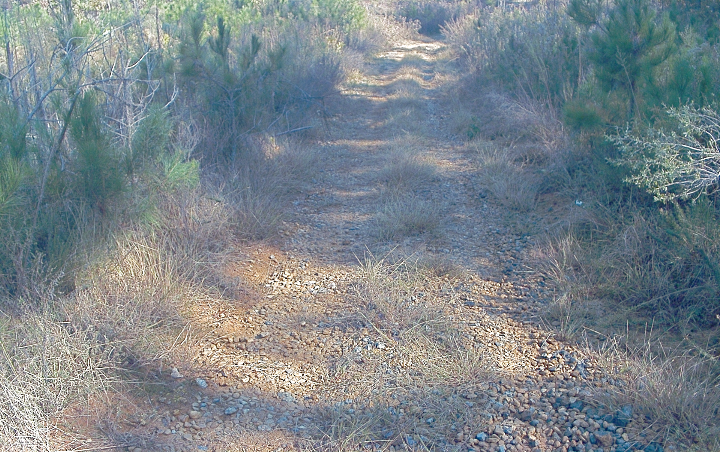
\includegraphics[width=\linewidth]{figures/qualitative/pidnet_detail_mixed_pln_961_rgb.png}
  \caption{RGB input.}
\end{subfigure}

\vspace{0.18cm}
\begin{subfigure}[t]{0.485\linewidth}
  \centering
  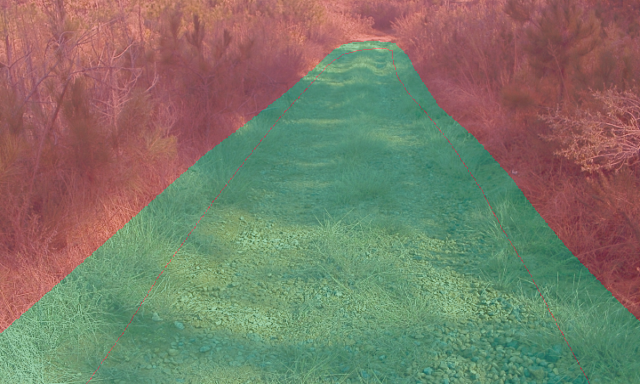
\includegraphics[width=\linewidth]{figures/qualitative/pidnet_detail_mixed_pln_961_gt.png}
  \caption{Ground-truth mapping.}
\end{subfigure}\hfill
\begin{subfigure}[t]{0.485\linewidth}
  \centering
  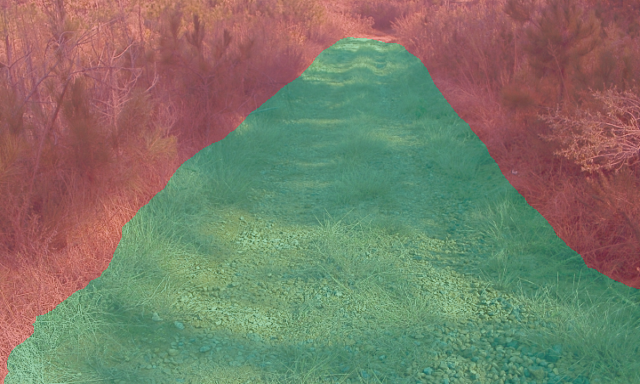
\includegraphics[width=\linewidth]{figures/qualitative/pidnet_detail_mixed_pln_961_prediction.png}
  \caption{PIDNet-S prediction.}
\end{subfigure}
\caption[Detailed successful winding-track example.]{Detailed view of
\texttt{mixed\_pln\_961}, the 10th-percentile example. The model follows the
winding foreground corridor into the distance. Its remaining 3.51\% FSR and
2.47\% FBR are concentrated primarily along the two lateral boundaries.}
\label{fig:pidnet_mapping_overlay}
\end{figure}

In Figure~\ref{fig:pidnet_mapping_overlay}, green extends along the track while
vegetation and terrain outside the selected vehicle envelope remain red. The
ground-truth and prediction overlays make small boundary offsets visible that
are difficult to see in the binary panels alone. The image connects the low
per-image rates to their spatial form.

\section{False-Safe, False-Block, and Boundary Failures}

\begin{figure}[H]
\centering
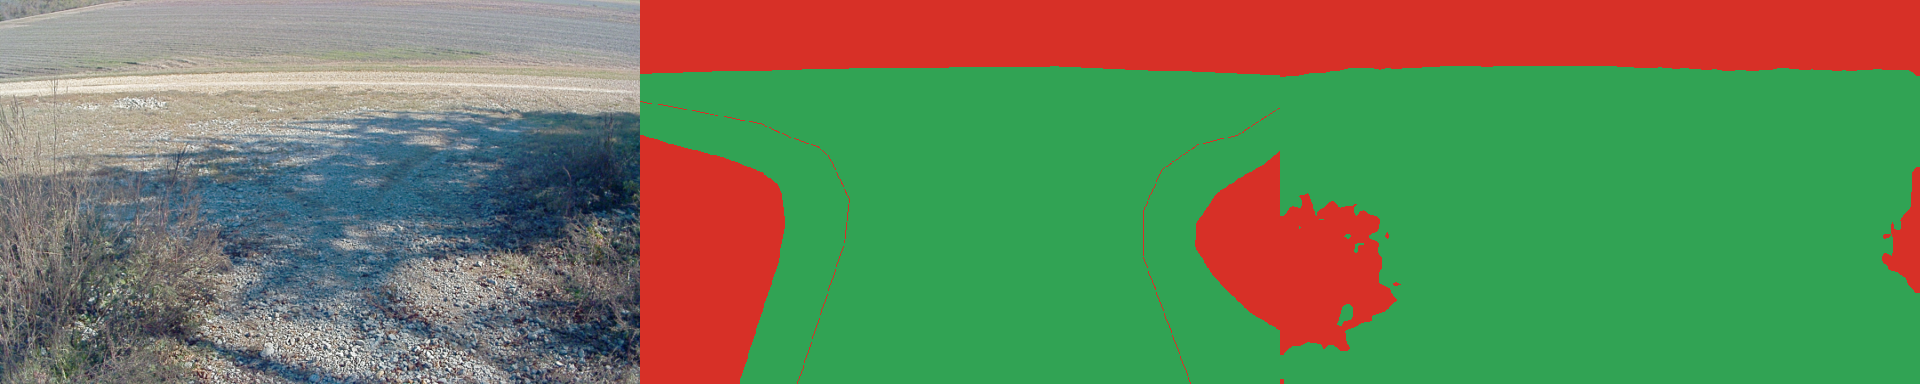
\includegraphics[width=0.96\linewidth]{figures/qualitative/pidnet_failure_false_safe_mixed_pln_1278.png}

\vspace{0.16cm}
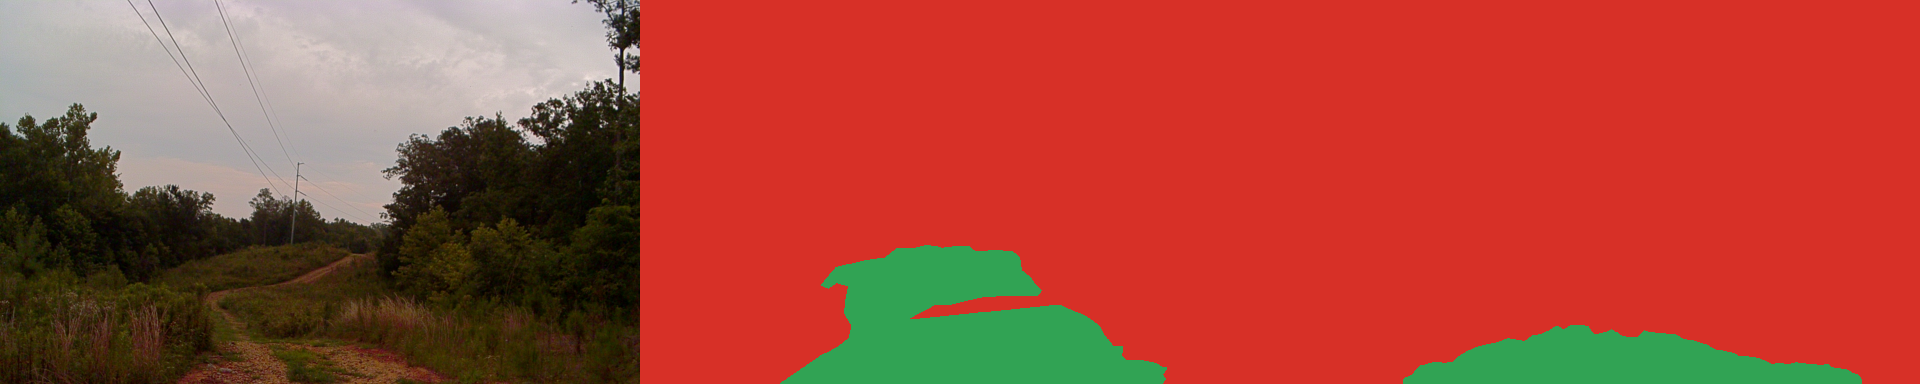
\includegraphics[width=0.96\linewidth]{figures/qualitative/pidnet_failure_false_block_mixed_425.png}

\vspace{0.16cm}
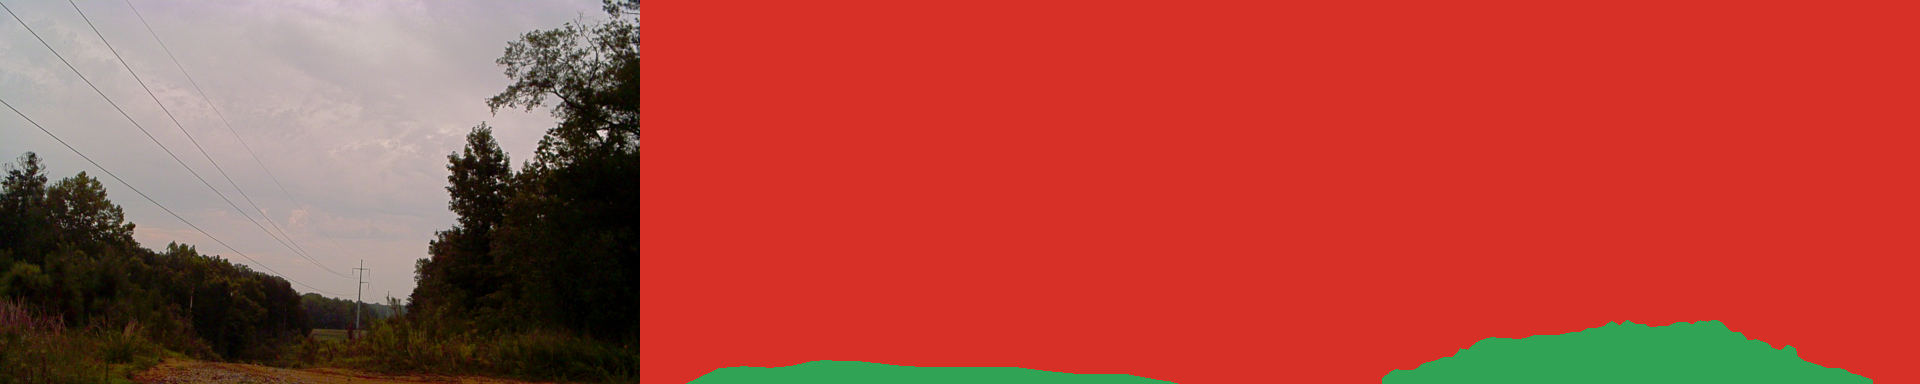
\includegraphics[width=0.96\linewidth]{figures/qualitative/pidnet_failure_boundary_mixed_459.png}
\caption[Asymmetric-error examples for reference PIDNet-S.]{Asymmetric-error
examples for reference PIDNet-S; each full-width triptych is RGB, ground truth, and
prediction. Top: \texttt{mixed\_pln\_1278}, maximum per-image FSR (30.20\%,
FBR 0.19\%). Middle: \texttt{mixed\_425}, maximum FBR (52.84\%, FSR 0.67\%).
Bottom: \texttt{mixed\_459}, 49.72\% boundary-band error (FSR 5.63\%, FBR
10.70\%).}
\label{fig:pidnet_failures}
\end{figure}

Figure~\ref{fig:pidnet_failures} provides the three ranked cases discussed
below: maximum FSR, maximum FBR, and severe boundary disagreement.

In the top case, the prediction opens almost the entire pale cultivated field
at the top and right of the image. The target admits the central and
foreground corridor but blocks that field under the blue+green policy. The
large connected green expansion explains the 30.20\% FSR; its spatial
coherence makes it more operationally important than the same number of
isolated pixels. The field and track share visual cues, so the example also
illustrates the annotation caveat: the model is clearly wrong relative to the
mask, but RGB alone does not reveal the physical property used to separate the
two capability regions.

In the middle case, the annotation marks a narrow path from the foreground
toward the left distance. The prediction retains only a small lower segment
and loses much of the shadowed corridor. This produces 52.84\% FBR but only
0.67\% FSR. It is conservative in the pixel convention, yet it could leave a
planner with no route. The weak distant contrast and narrow labelled geometry
connect the visible failure to the numerical rate.

The bottom case contains an irregular interface between low vegetation and
track. The prediction moves the foreground contour and changes the width of
the feasible strip. The global FSR and FBR are not as extreme, but nearly half
of the four-pixel-wide target boundary band is wrong. Because more than one
nearby contour can look plausible at this interface, the 49.72\% result should
be interpreted as precise disagreement with the supplied annotation, not as a
measurement of physical clearance error.

Together, the examples show three different remediation targets. False-safe
expansion suggests stronger physical cues, calibration, or planner-side
constraints. False blocks suggest better recall for narrow and shadowed
corridors. Boundary disagreement suggests boundary-aware supervision,
higher-quality annotation, or planning margins. A single loss change is
unlikely to address all three.

\section{Qualitative Transfer to ALICE}

\begin{figure}[H]
\centering
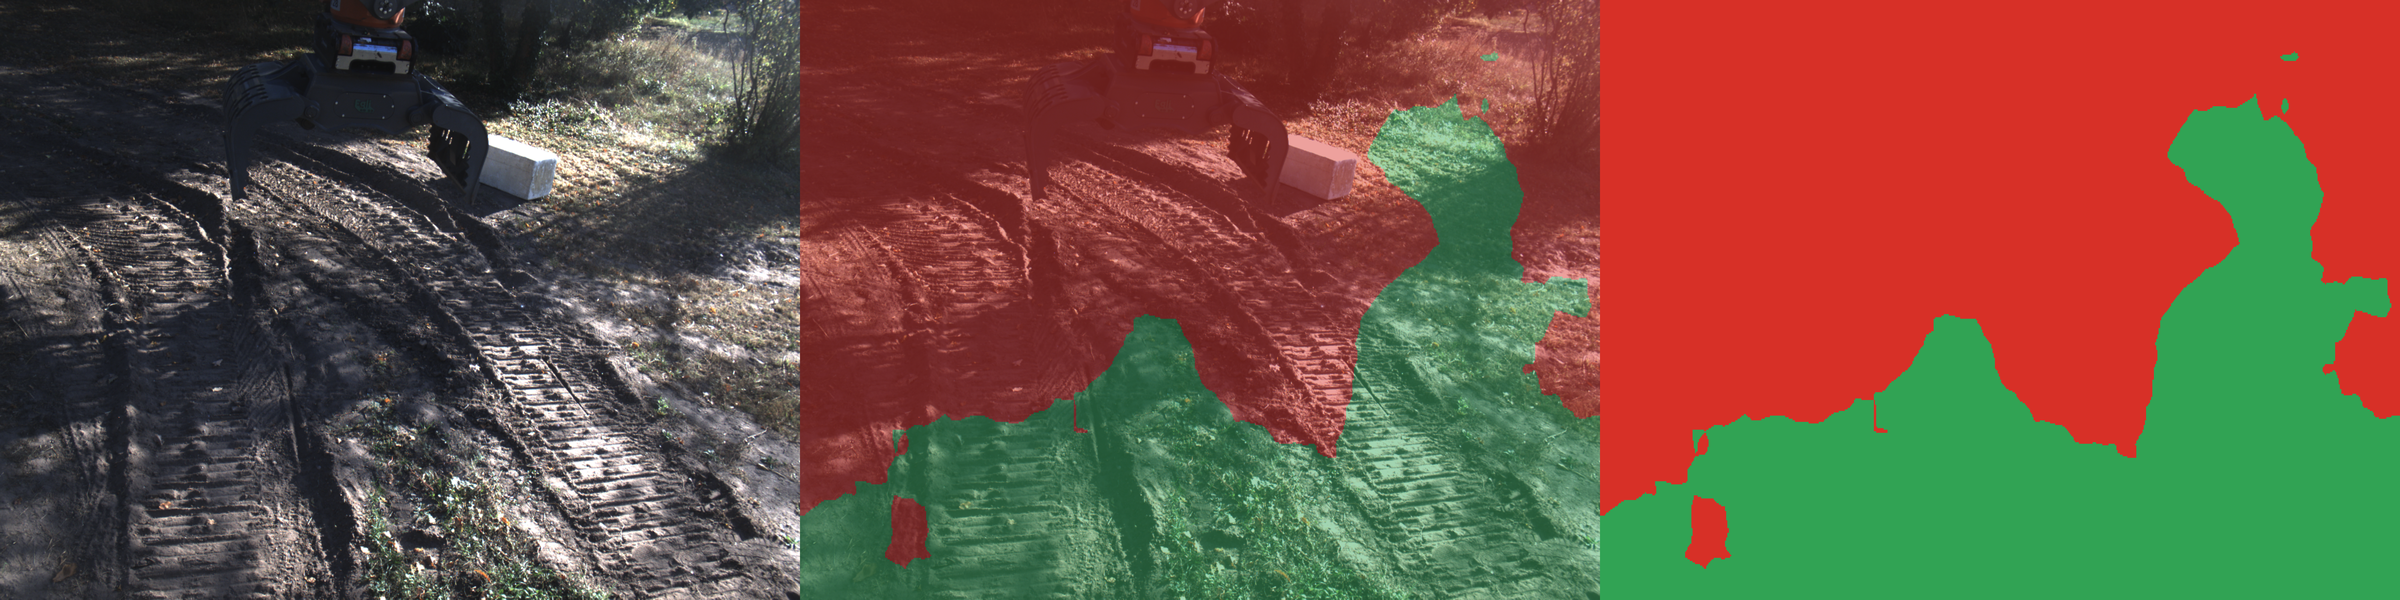
\includegraphics[width=0.96\linewidth]{figures/qualitative/pidnet_alice_sequence01.png}

\vspace{0.12cm}
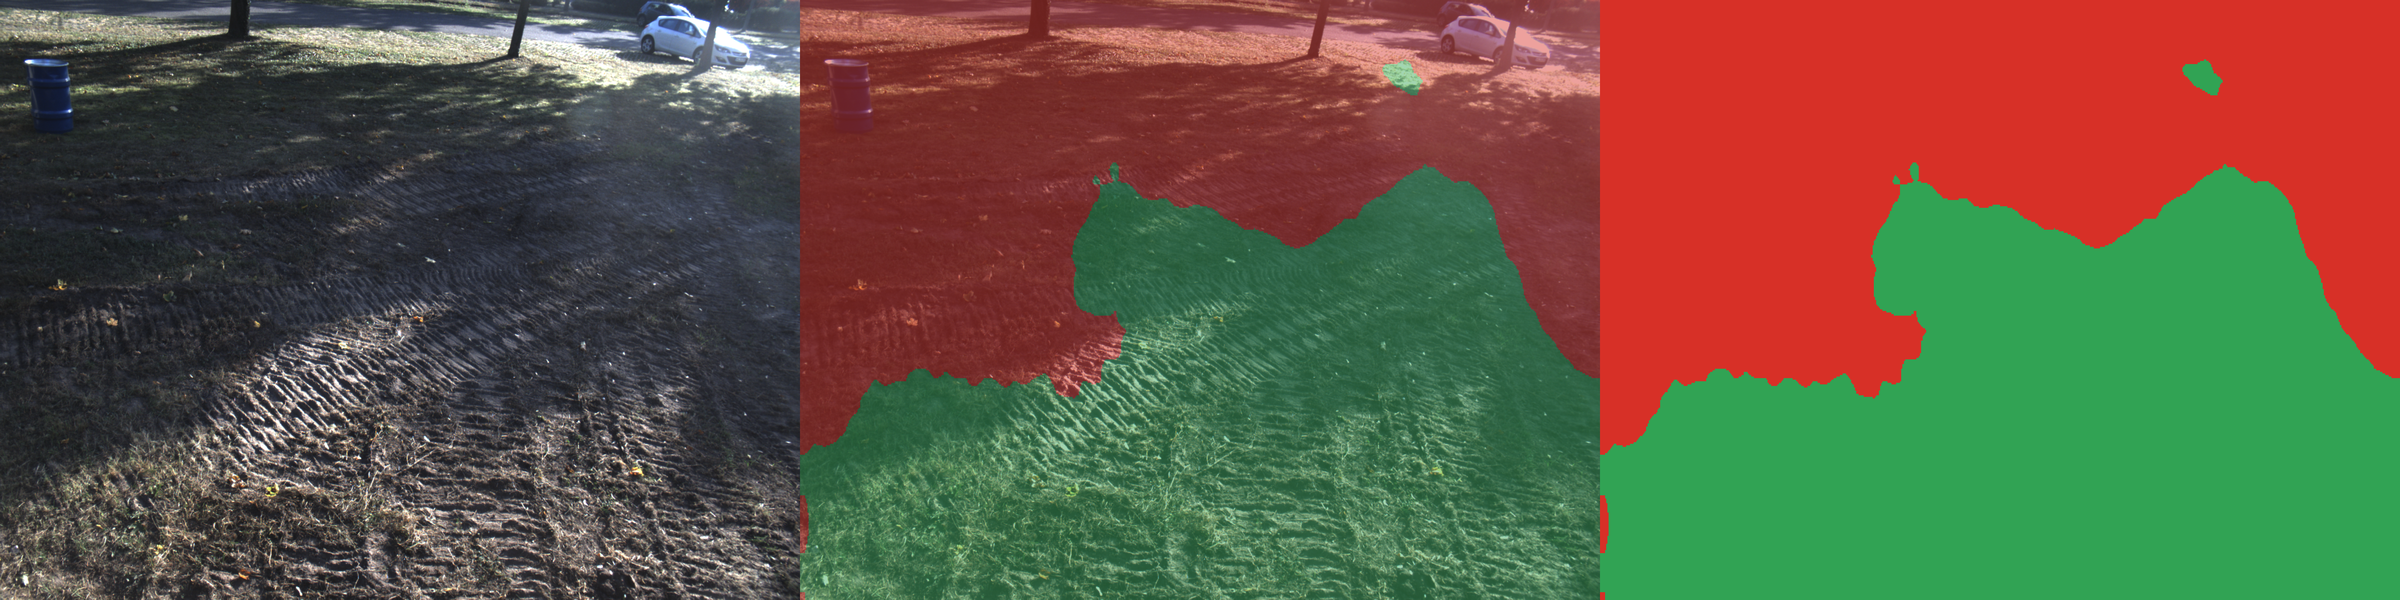
\includegraphics[width=0.96\linewidth]{figures/qualitative/pidnet_alice_sequence02.png}

\vspace{0.12cm}
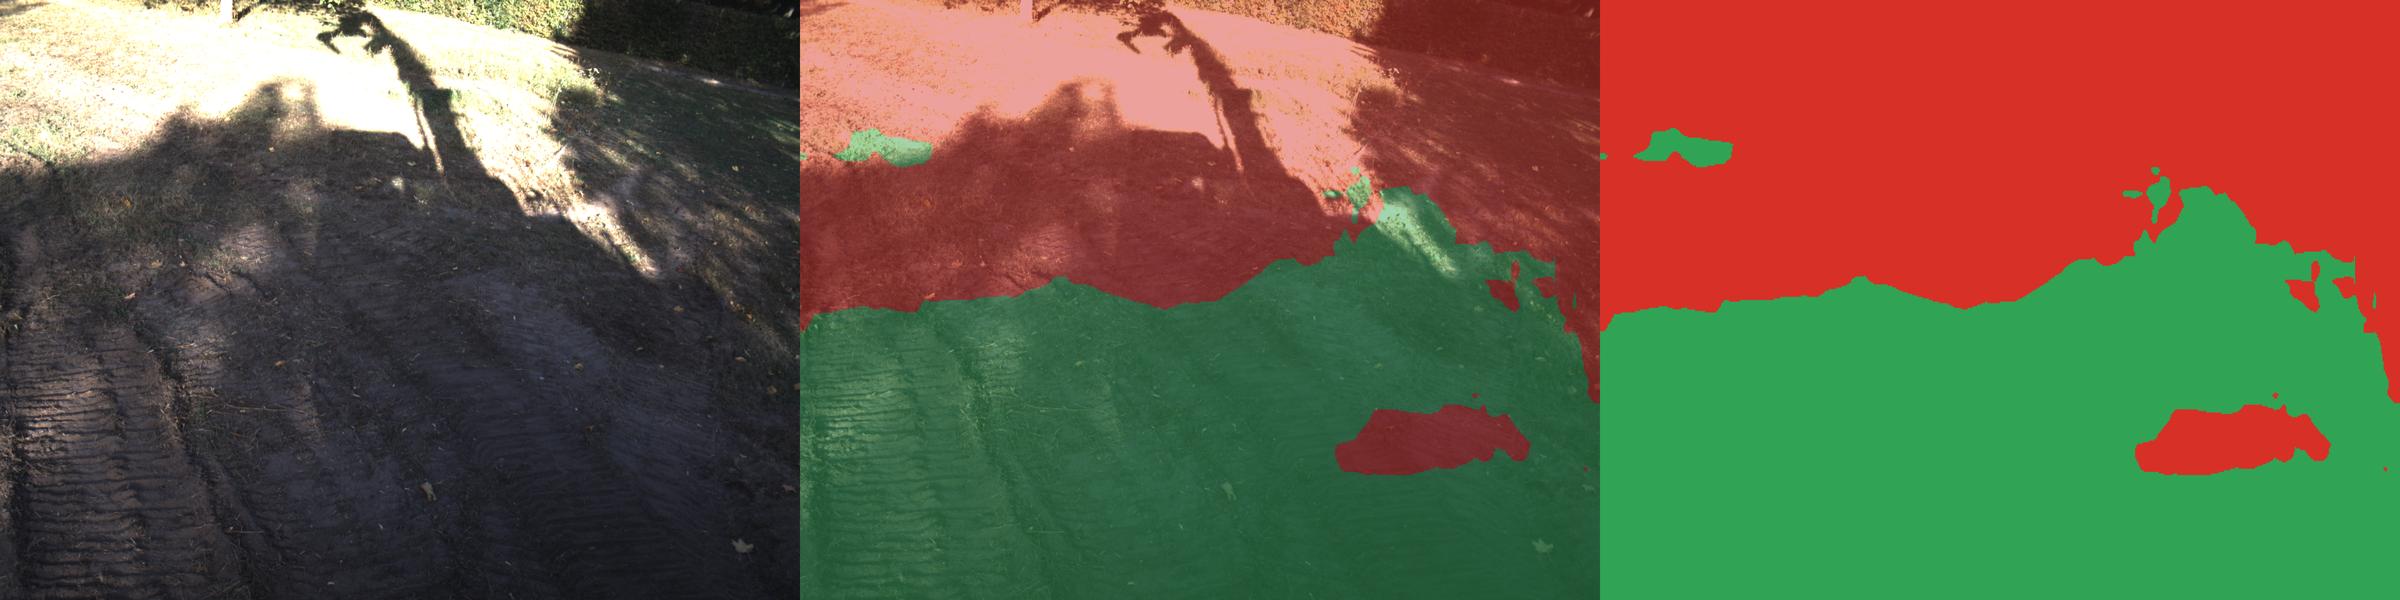
\includegraphics[width=0.96\linewidth]{figures/qualitative/pidnet_alice_sequence04.png}

\vspace{0.12cm}

\includegraphics[width=0.96\linewidth]{figures/qualitative/pidnet_alice_sequence05.png}
\caption[Unscored PIDNet-S transfer to ALICE.]{Unscored transfer of the same
reference blue+green PIDNet-S checkpoint to the external ALICE mobile-robot
sequences. Each triptych shows RGB input, prediction overlay, and binary
prediction. No ALICE ground truth is available, so the panels show output
behaviour only.}
\label{fig:alice_transfer}
\end{figure}

Figure~\ref{fig:alice_transfer} is intentionally qualitative: it shows how the
fixed checkpoint responds to external scenes but supplies no accuracy claim.

The first ALICE frame contains another robot close to the camera. The model
mostly blocks the robot body and produces a narrow irregular traversable
region below and around it, showing that the output responds to a foreground
object rather than blindly opening the entire image. The second frame contains
grass, shadows, a paved road, a parked car, and a barrel. The prediction opens
a foreground grass wedge while largely blocking the road at the top. This is a
warning that a CaT-trained capability prior is not a general road detector.

The third frame has severe illumination contrast. The model forms a broad
foreground region but introduces holes and fragments near shadow boundaries.
The fourth frame contains a visible central worn track through leaf-covered
ground; the prediction forms a large connected lower region aligned only
partly with that visual track. Across the four scenes the masks are structured
and change with scene content, but their apparent plausibility varies.

No statement such as ``the model generalises to ALICE'' can be derived from
these images. There is no target mask, no vehicle trial, and no calibration
measurement. The panels only demonstrate that the reference pipeline executes on
the new camera data and reveal concrete behaviours that a future labelled
ALICE study should score.
